%%%%%%%%%%%%%%%%%%%%%%%%%%%%%%%%%%%%%%%%%
% Large Colored Title Article
% LaTeX Template
% Version 1.1 (25/11/12)
%
% This template has been downloaded from:
% http://www.LaTeXTemplates.com
%
% Original author:
% Frits Wenneker (http://www.howtotex.com)
%
% License:
% CC BY-NC-SA 3.0 (http://creativecommons.org/licenses/by-nc-sa/3.0/)
%
%%%%%%%%%%%%%%%%%%%%%%%%%%%%%%%%%%%%%%%%%

%----------------------------------------------------------------------------------------
%	PACKAGES AND OTHER DOCUMENT CONFIGURATIONS
%----------------------------------------------------------------------------------------

\documentclass[DIV=calc, paper=a4, fontsize=10pt, twocolumn]{scrartcl}	 % A4 paper and 11pt font size

\usepackage{lipsum} % Used for inserting dummy 'Lorem ipsum' text into the template
\usepackage{url}
\usepackage{natbib}
\usepackage[english]{babel} % English language/hyphenation
\usepackage[protrusion=true,expansion=true]{microtype} % Better typography
\usepackage{amsmath,amsfonts,amsthm} % Math packages
\usepackage[svgnames]{xcolor} % Enabling colors by their 'svgnames'
\usepackage[hang, small,labelfont=bf,up,textfont=it,up]{caption} % Custom captions under/above floats in tables or figures
\usepackage{booktabs} % Horizontal rules in tables
\usepackage{fix-cm}	 % Custom font sizes - used for the initial letter in the document
\usepackage{natbib}
\usepackage{sectsty} % Enables custom section titles
\allsectionsfont{\usefont{OT1}{phv}{b}{n} \fontsize{12}{12}} % Change the font of all section commands
\usepackage{hyperref}
\usepackage{float}
\usepackage{fancyhdr} % Needed to define custom headers/footers
\pagestyle{fancy} % Enables the custom headers/footers
\usepackage{lastpage} % Used to determine the number of pages in the document (for "Page X of Total")

% Headers - all currently empty
\lhead{}
\chead{\emph{A User-Friendly U.S. Census Browser for R}}
\rhead{}

% Footers
\lfoot{}
\cfoot{}
\rfoot{\footnotesize Page \thepage\ of \pageref{LastPage}} % "Page 1 of 2"

\renewcommand{\headrulewidth}{0.0pt} % No header rule
\renewcommand{\footrulewidth}{0.4pt} % Thin footer rule

\usepackage{lettrine} % Package to accentuate the first letter of the text
\newcommand{\initial}[1]{ % Defines the command and style for the first letter
\lettrine[lines=3,lhang=0.3,nindent=0em]{
\color{black}
{\textsf{#1}}}{}}
\usepackage{color}
\definecolor{purple}{rgb}{.4,0,.8}
\newcommand{\hh}[1]{{\color{magenta} #1}}
\newcommand{\st}[1]{{\color{purple} #1}}

%----------------------------------------------------------------------------------------
%	TITLE SECTION
%----------------------------------------------------------------------------------------

\usepackage{titling} % Allows custom title configuration

\newcommand{\HorRule}{\color{black} \rule{\linewidth}{1pt}} % Defines the gold horizontal rule around the title

\pretitle{\vspace{-50pt} \begin{flushleft} \HorRule \fontsize{15}{15} \usefont{OT1}{phv}{b}{n} \color{black} \selectfont} % Horizontal rule before the title

\title{\texttt{censusbrowseR}: A User-Friendly U.S. Census Browser for R} % Your article title
 % This should probably reference geomnet. Don't want it to be too long though
\posttitle{\par\end{flushleft}\vskip 0em} % Whitespace under the title

\preauthor{\begin{flushleft}\large \vspace{-.5cm} \usefont{OT1}{phv}{b}{sl} \color{black}} % Author font configuration

\author{Kiegan Rice, } % Your name

\postauthor{\footnotesize \usefont{OT1}{phv}{m}{sl} \color{Black} % Configuration for the institution name
Iowa State University % Your institution

\par\end{flushleft} \vspace{-.5cm} \HorRule \vspace{-1cm}} % Horizontal rule after the title
\date{} % Add a date here if you would like one to appear underneath the title block

%----------------------------------------------------------------------------------------

\usepackage{Sweave}
\begin{document}
\Sconcordance{concordance:ASA_SCSG_writeup.tex:ASA_SCSG_writeup.Rnw:%
1 198 1 50 0 1 25 11 1 1 14 14 1 1 39 11 1 1 58 9 1 1 68 12 1 1 66 %
28 1}

%\SweaveOpts{concordance=TRUE}
\setkeys{Gin}{width=0.5\textwidth}


\maketitle % Print the title

\thispagestyle{fancy} % Enabling the custom headers/footers for the first page 

%----------------------------------------------------------------------------------------
%	ABSTRACT
%----------------------------------------------------------------------------------------

% The first character should be within \initial{}
\vspace{-1cm}
%\initial{U}\textbf{sing a new way to visualize network data in \texttt{R} with \texttt{gglot2}, I examine the evolution of the African slave trade from the $16^{th}$ through the $19^{th}$ centuries. \st{XXX I feel like I need more here. Will add more when paper is more fleshed out.}}

%\initial{T}\textbf{he Trans-Atlantic Slave Trade Database, hosted by Emory University, contains information on nearly 35,000 voyages of slave ships from 1514 - 1866 between Europe, Africa, and the Americas. The entire database contains 279 variables with information on the 34,948 voyages. While the website dedicated to this data contains a dashboard to subset and visualize the data, I wanted to view the data in a new way. I use the \texttt{geomnet} package because I wanted to show that the user can visually explore the data in a way that leaves them with a deeper understanding of the structure of the slave trade. I start by visualizing all of the data I pulled from the database on one map, then I look at different subsets of it, and I end with a much deeper understanding of the slave trade and its impact on the world.}
%----------------------------------------------------------------------------------------
%	ARTICLE CONTENTS
%----------------------------------------------------------------------------------------
\section*{Introduction}

\initial{C}ensus data provide an important snapshot of information about a country at different times throughout its history, and their value is difficult to overstate.  While history books present a narrative of the events that occured, students themselves often don't get to interact with the raw data in that learning environment. Clean and accessible census data allow the exploration of different demographic groups over time, or investigations of a particular period of time and what the demographic and economic landscape looked like in the past. Even today, data about the world around us opens a pathway for learning more about places we haven't been and groups of people with whom we may not usually engage.  

\par From an early point in the United States' history, there were many "eminent men of science" who recognized the value of the census data and worked to aggregate and present those data. Francis A. Walker's "Statistical Atlas of the United States", based on the 1870 census, was an impressive effort in aggregating population data to present them in a visually appealing way \citep{StatisticalAtlas}. Although the Census Bureau's "Statistical Atlases" eventually stopped being created, they were an important start to the effort of visually presenting census data to a wider public (see~\autoref{atlas}).

\begin{center}
\includegraphics[width=6cm]{./figures/colored-population-stat-atlas.png}  
\captionof{figure}{A visualization of the African American population in the United States from the ``Statistical Atlas of the United States".}\label{atlas}
\end{center}

\par Today, as methods of data analysis and visualization continue to be developed and improved, access to census data allows us to look back on that history and explore, synthesize, and visualize the information. When aggregated and presented in a clear manner, viewers can learn more about patterns in many different parts of the population. A 2007 paper about the Statistical Atlas discusses just how much information is present in those original charts and demonstrates several other ways of presenting the information that can be found therein \citep{ChartInterview}.  

\par Ever-improving visualization and data-wrangling methods in R \citep{RCoreTeam} give those interested in statistical graphics a wealth of opportunities to explore and learn from data; in particular, incorporating user interactivity using Shiny has revolutionized the way statisticians share and communicate information \citep{Shiny}. However, it is difficult to make use of these tools with census data if those data are not available and easy to explore in one location.  

\par An inherent problem in census data is that a country's census changes over time; the variables collected, how they are collected, and even the locations on which they are collected are updated as the country is formed, and subsequently grows and changes. The United States census data are no exception to this rule. In little under two and a half centuries, the census has taken many different forms. Data on occupations have transformed as the employment landscape has changed; new states have been formed, the most recent being within the last 100 years; definitions of various demographic groups and the terminology used to describe them have been updated as the demographic makeup of the country has changed. Each decennial census brings a different set of variables to the table. Sometimes these variables are new things the Census Bureau is interested in learning about, while sometimes they remove variables that are no longer relevant or whose information is captured elsewhere.  

\par Unfortunately, because the founders of the U.S. Census were unable to see 200 years into the future, those interested in working with census data are left with quite the inescapable mess. If you want to focus in on a particular demographic group and their journey as part of the population of the United States, you may have ten or more different variable names to describe that one group over the course of the census from 1790 to 1960 - and that is just for a single group! Of course, we cannot just simply change variable names to match our own research needs. It is important to keep the data in their true form and be respectful of the way in which the population was defined at different times throughout history, even if our instinct may be to 'clean' the data by changing variable names.  

\par This, of course, leaves the user with a wide variety of variables that are far from consistent across years. In order to track one demographic group across years - let alone many groups - a clean user interface that helps users see exactly what information is available to them is a necessity. To streamline the process and assist researchers in finding out to what information they have access and what information they lack, a U.S. Census Browser for R is presented as an R package, with the user interface being a Shiny application, and the downloadable files being 'tidy' comma-separated values (csv) files that those with a minimal amount of R experience can still process.  
%------------------------------------------------




\section*{Data Access}  

\section*{The \texttt{censusbrowseR} package}  

After ordering by how many years each variable appears in, the available variable names show a serious lack of continuity. The four ever-present variables (\texttt{Year}, \texttt{State}, \texttt{TOTAL.POPULATION}, and \texttt{Type}) each appear ten times, once in each year selected. After that, the next most common variable only appears in four of the ten years we have chosen. This highlights some of the hurdles that we will encounter when tracking any demographic group over time. 

Since the focus will be on African Americans throughout U.S. history, the first search term needed is \texttt{SLAVE} in the early years of the U.S. census. The vast majority of African Americans were slaves when the United States was founded, so variables that count the number of slaves tell the story about the African American population in early U.S. history. Note that the `SLAVE` categorization is the only term the U.S. census had related to African Americans in the early years of the census, so it is also the only source of information available on that group for that time period.  



\begin{figure}
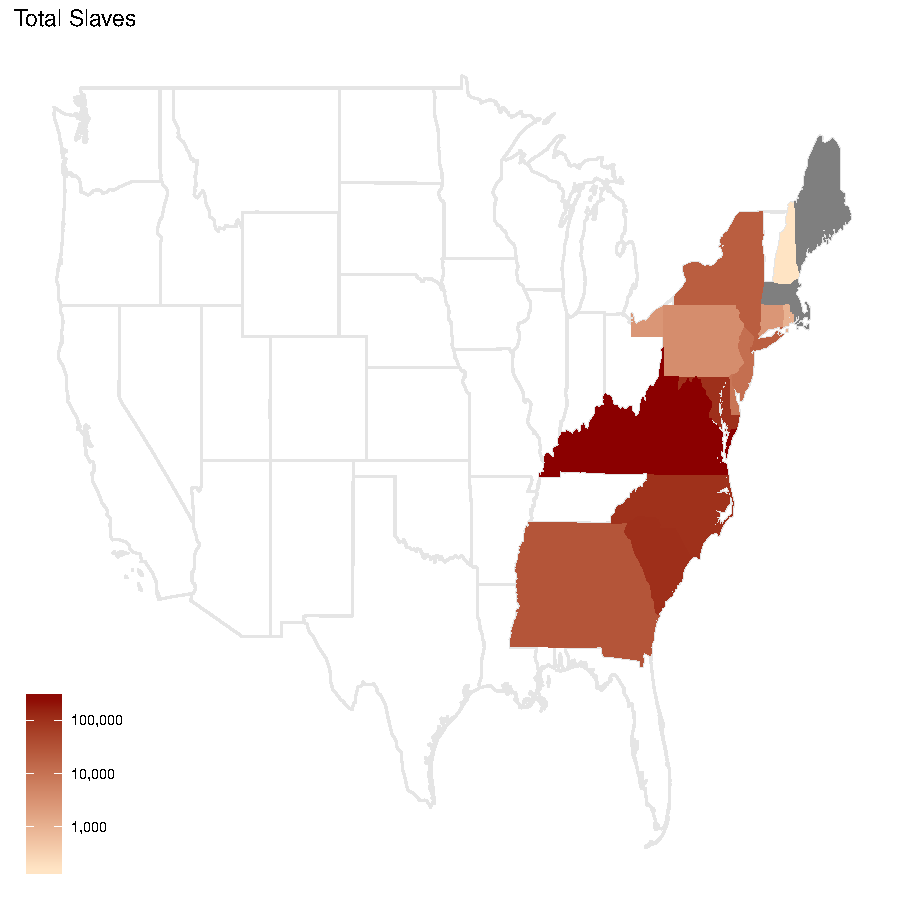
\includegraphics{ASA_SCSG_writeup-002}
\caption{Total number of slaves per state in 1790, plotted on a continuous log scale. State boundaries for July 4, 1790 were gathered from `USAboundaries` package.}
\label{map_1790}
\end{figure}

Blah blah blah \autoref{map_1790} is important.





\section*{Conclusion}
The decennial census is a rich source of historical information. We have built a tool that can help extract and visualize that information to, for example, understand how demographic attributes of the U.S. population have changed over time.  

Although there is no county-level information available and the data for the census browser go only through 1960, users are able to efficiently explore variables of interest at different time points in U.S. history and tell a visual story about a growing nation and a changing population. This connectivity across years and ability to assess what information was available when, all in one browser, have the potential to save time and effort of researchers interested in delving into United States history.

The structure of our browsers also helps determine not only the variables that are available in a given year, but also where information is missing for some states on a particular variable. Finding these differences is easier when all relevant variables are combined in one data frame, which can be summarized and searched all at one time. 
%----------------------------------------------------------------------------------------
%	REFERENCE LIST
%----------------------------------------------------------------------------------------
\bibliographystyle{abbrv}
\bibliography{bibliography}
\section*{Further Reading}


%----------------------------------------------------------------------------------------

\end{document}
